% !TEX root = Bachelorarbeit Synthetische Daten.tex
\chapter{Ergebnisse} \label{sec:results}

Dieses Kapitel präsentiert die Ergebnisse der Arbeit. Es wird auf die generierten synthetischen Daten eingegangen und die Trainings- und Testergebnisse der Modelle beschrieben. Anschließend wird die Klassifikations-Performance der Modelle verglichen und die Out-of-Distribution-Detektion analysiert.

\section{Die generierten synthetischen Daten} \label{sec:da-fusion-results}

% Einleitung/Überblick
Im Folgenden werden die generierten synthetischen Daten vorgestellt, aufgeteilt in In-Distribution- und Near Out-of-Distribution-Augmentationen. Es wird auf die Qualität der Daten durch menschliche Evaluierung eingegangen. Die Generierung wurde im vorherigen Kapitel im Detail behandelt (siehe Abschnitt \ref{sec:da-fusion-setup}).

% Validation Images; stetiges Verbessern (Gemeinsames Finetuning)

\subsection{In-Distribution} \label{sec:da-fusion-id-results}

In Abbildung \ref{fig:id-augs-detail-good} sind Beispiele der synthetischen In-Distribution-Daten zu sehen. Die Bilder sind überwiegend sehr überzeugend und realistisch. Da der \lstinline{strength}-Parameter der Augmentationen auf 0.2 gesetzt wurde, sind die Unterschiede subtil, aber dennoch sichtbar. Die Form und Struktur der Objekte blieb erhalten, während Veränderungen in der Textur der Oberflächen erkennbar sind.

\begin{figure}[h]
	\centering
	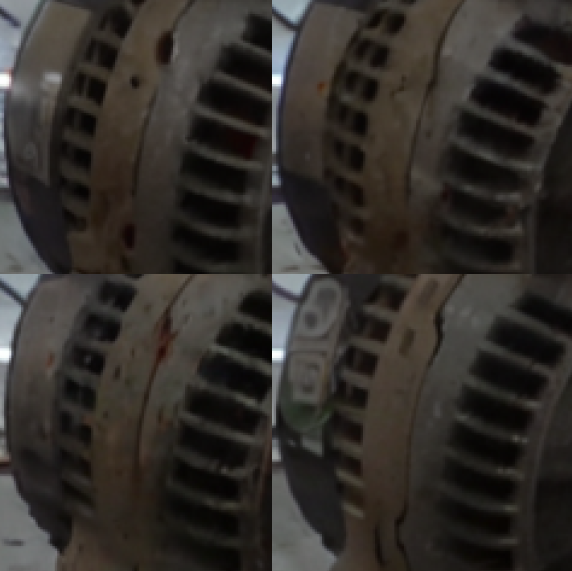
\includegraphics[width=0.5\textwidth]{figure_results_id-augs_detail_1.png}%
	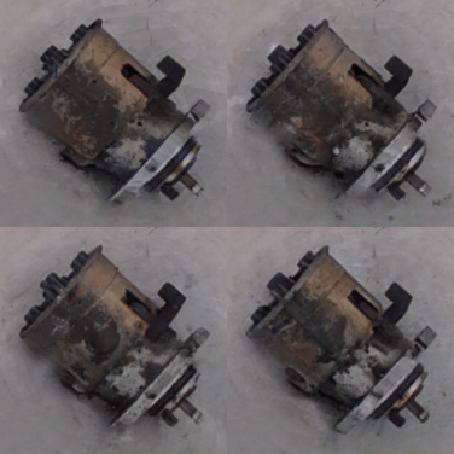
\includegraphics[width=0.5\textwidth]{figure_results_id-augs_detail_2.png}
	\caption{Vergrößerte Ausschnitte der synthetischen In-Distribution-Daten.}
	\label{fig:id-augs-detail-good}
\end{figure}

In einigen Fällen sind die Ergebnisse jedoch weniger überzeugend. In Abbildung \ref{fig:id-augs-detail-bad} sind Beispiele für mangelhafte In-Distribution-Daten zu sehen. Die synthetischen Objekte sind in diesen Fällen nicht realistisch und weisen deutliche Artefakte auf. Die Qualität der Daten hängt dabei nicht nur von der Art des Objekts, sondern auch von der Größe des Objektes im Originalbild (was auch die Auflösung des ROI-Crops entscheidet). Bei glatten Oberflächen und einfachen Formen sind die Ergebnisse besser als bei komplexen Strukturen und unregelmäßigen Oberflächen.

\begin{figure}[h]
	\centering
	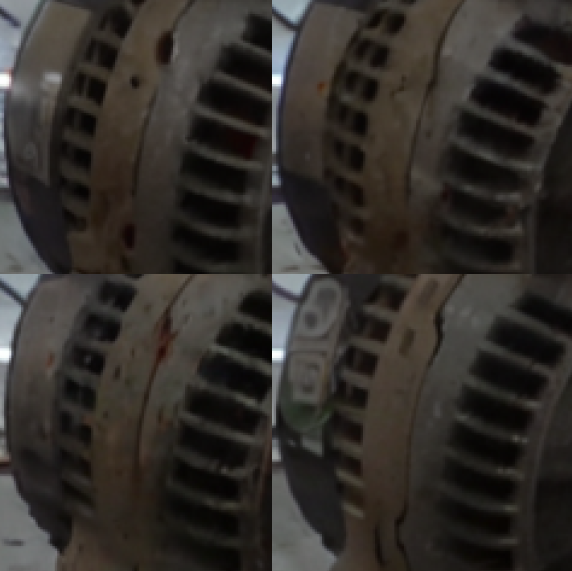
\includegraphics[width=0.5\textwidth]{figure_results_id-augs_detail_1.png}%
	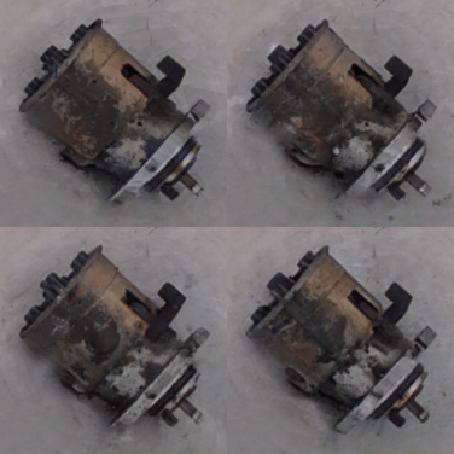
\includegraphics[width=0.5\textwidth]{figure_results_id-augs_detail_2.png}
	\caption{Beispiele für mangelhafte In-Distribution-Daten.}
	\label{fig:id-augs-detail-bad}
\end{figure}

\subsection{Near Out-of-Distribution} \label{sec:da-fusion-ood-results}

Die synthetischen Near Out-of-Distribution-Daten sind in Abbildung \ref{} dargestellt. Die Qualität der Daten ist insgesamt etwas schlechter als bei den In-Distribution-Daten, was auf Grund des größeren \lstinline{strength}-Parameters von 0.5 zu erwarten war. Die Objekte wirken weniger realistisch, aber dennoch plausibel. Die Wirksamkeit der Beispiele im Training kann jedoch an dieser Stelle noch nicht beurteilt werden.

%\begin{figure}[h]
%	\centering
%	\includegraphics[width=0.5\textwidth]{figure_results_ood-augs_detail_1.png}%
%	\includegraphics[width=0.5\textwidth]{figure_results_ood-augs_detail_2.png}
%	\caption{Beispiele der synthetischen Near Out-of-Distribution-Daten.}
%	\label{fig:ood-augs-detail}
%\end{figure}

\section{Trainings- und Testergebnisse} \label{sec:supcon-results}

% Einleitung
Es werden nun die Ergebnisse der Trainings- und Testdurchläufe im Supervised Contrastive Learning beschrieben. Es wird auf die Trainingskurven und die Performance der Modelle eingegangen.

\subsection{Contrastive Pre-Training} \label{sec:supcon-pre-results}

Abbildung \ref{fig:supcon-pre-loss} zeigt die Trainingskurven des Contrastive Pre-Trainings. Die Trainings- und Validierungsfehler zeigen insgesamt eine gute Konvergenz. Die Validierungskurve zeigt eine leichte Überanpassung, was auf eine gute Generalisierungsfähigkeit des Modells hindeutet. Die Trainingskurve zeigt eine leichte Oszillation, was auf eine gute Lernrate hindeutet.

\begin{figure}[h]
	\centering
	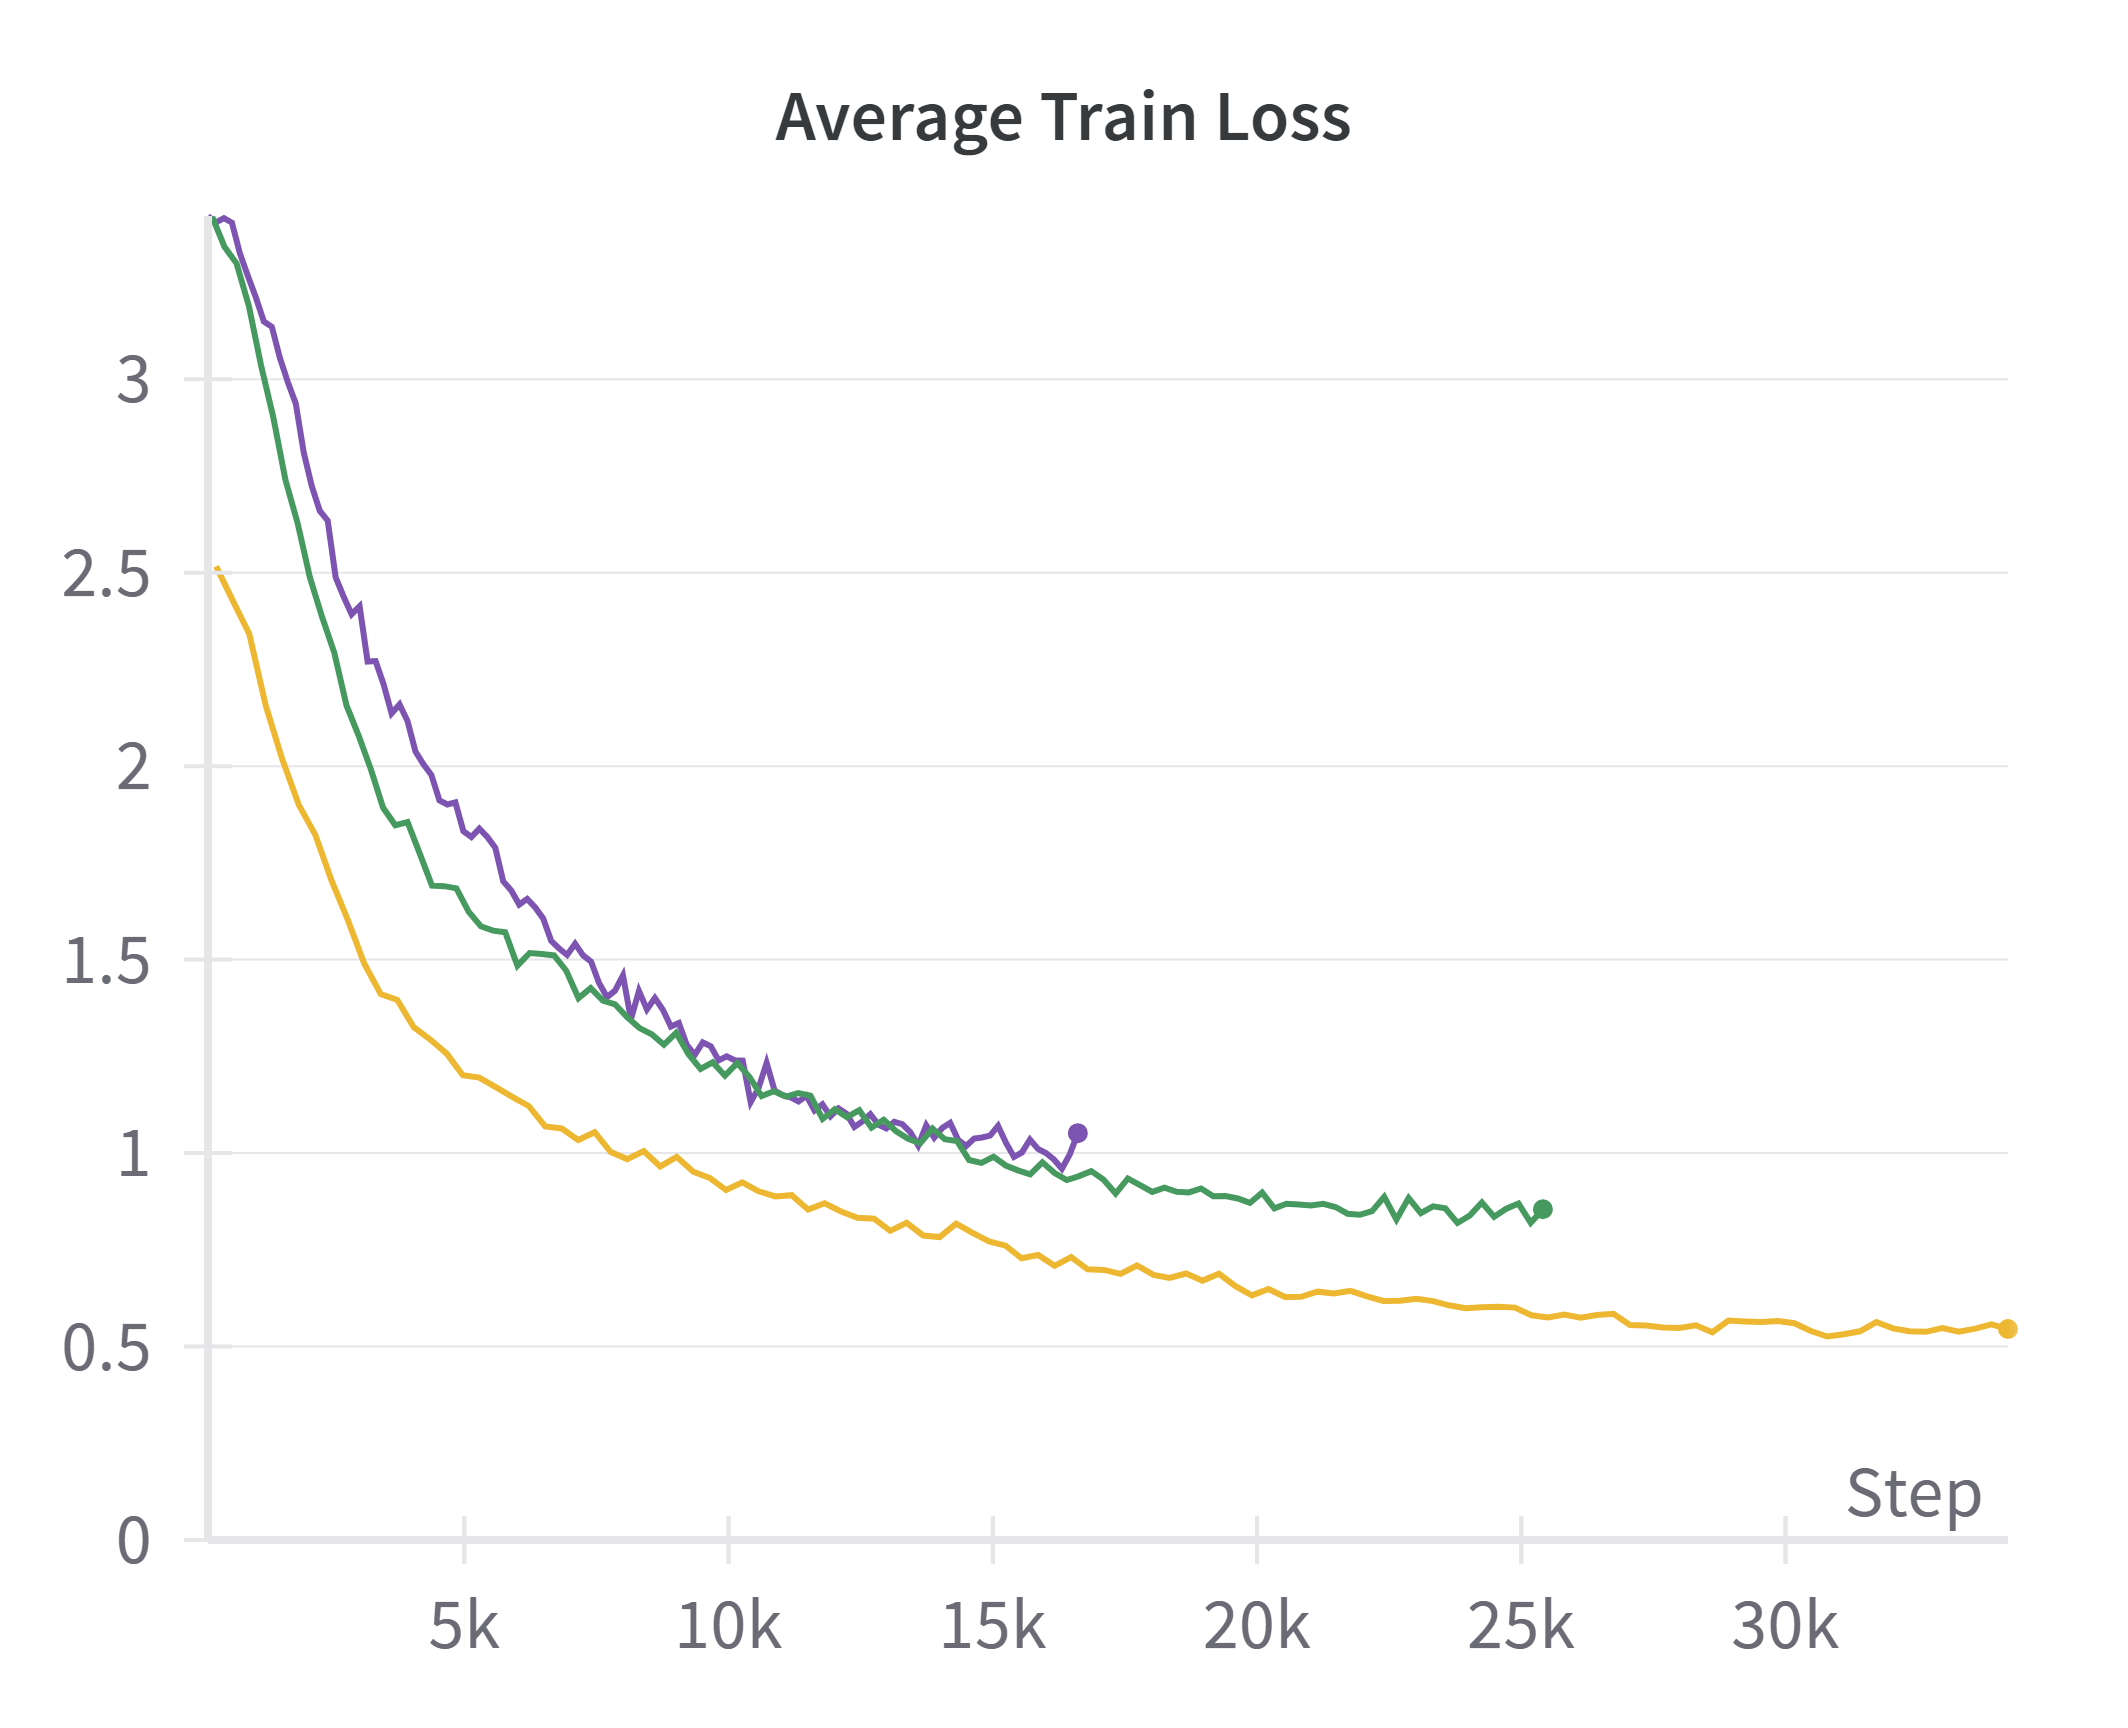
\includegraphics[width=0.5\textwidth]{figure_results_supcon-pre_avg-train-loss.png}%
	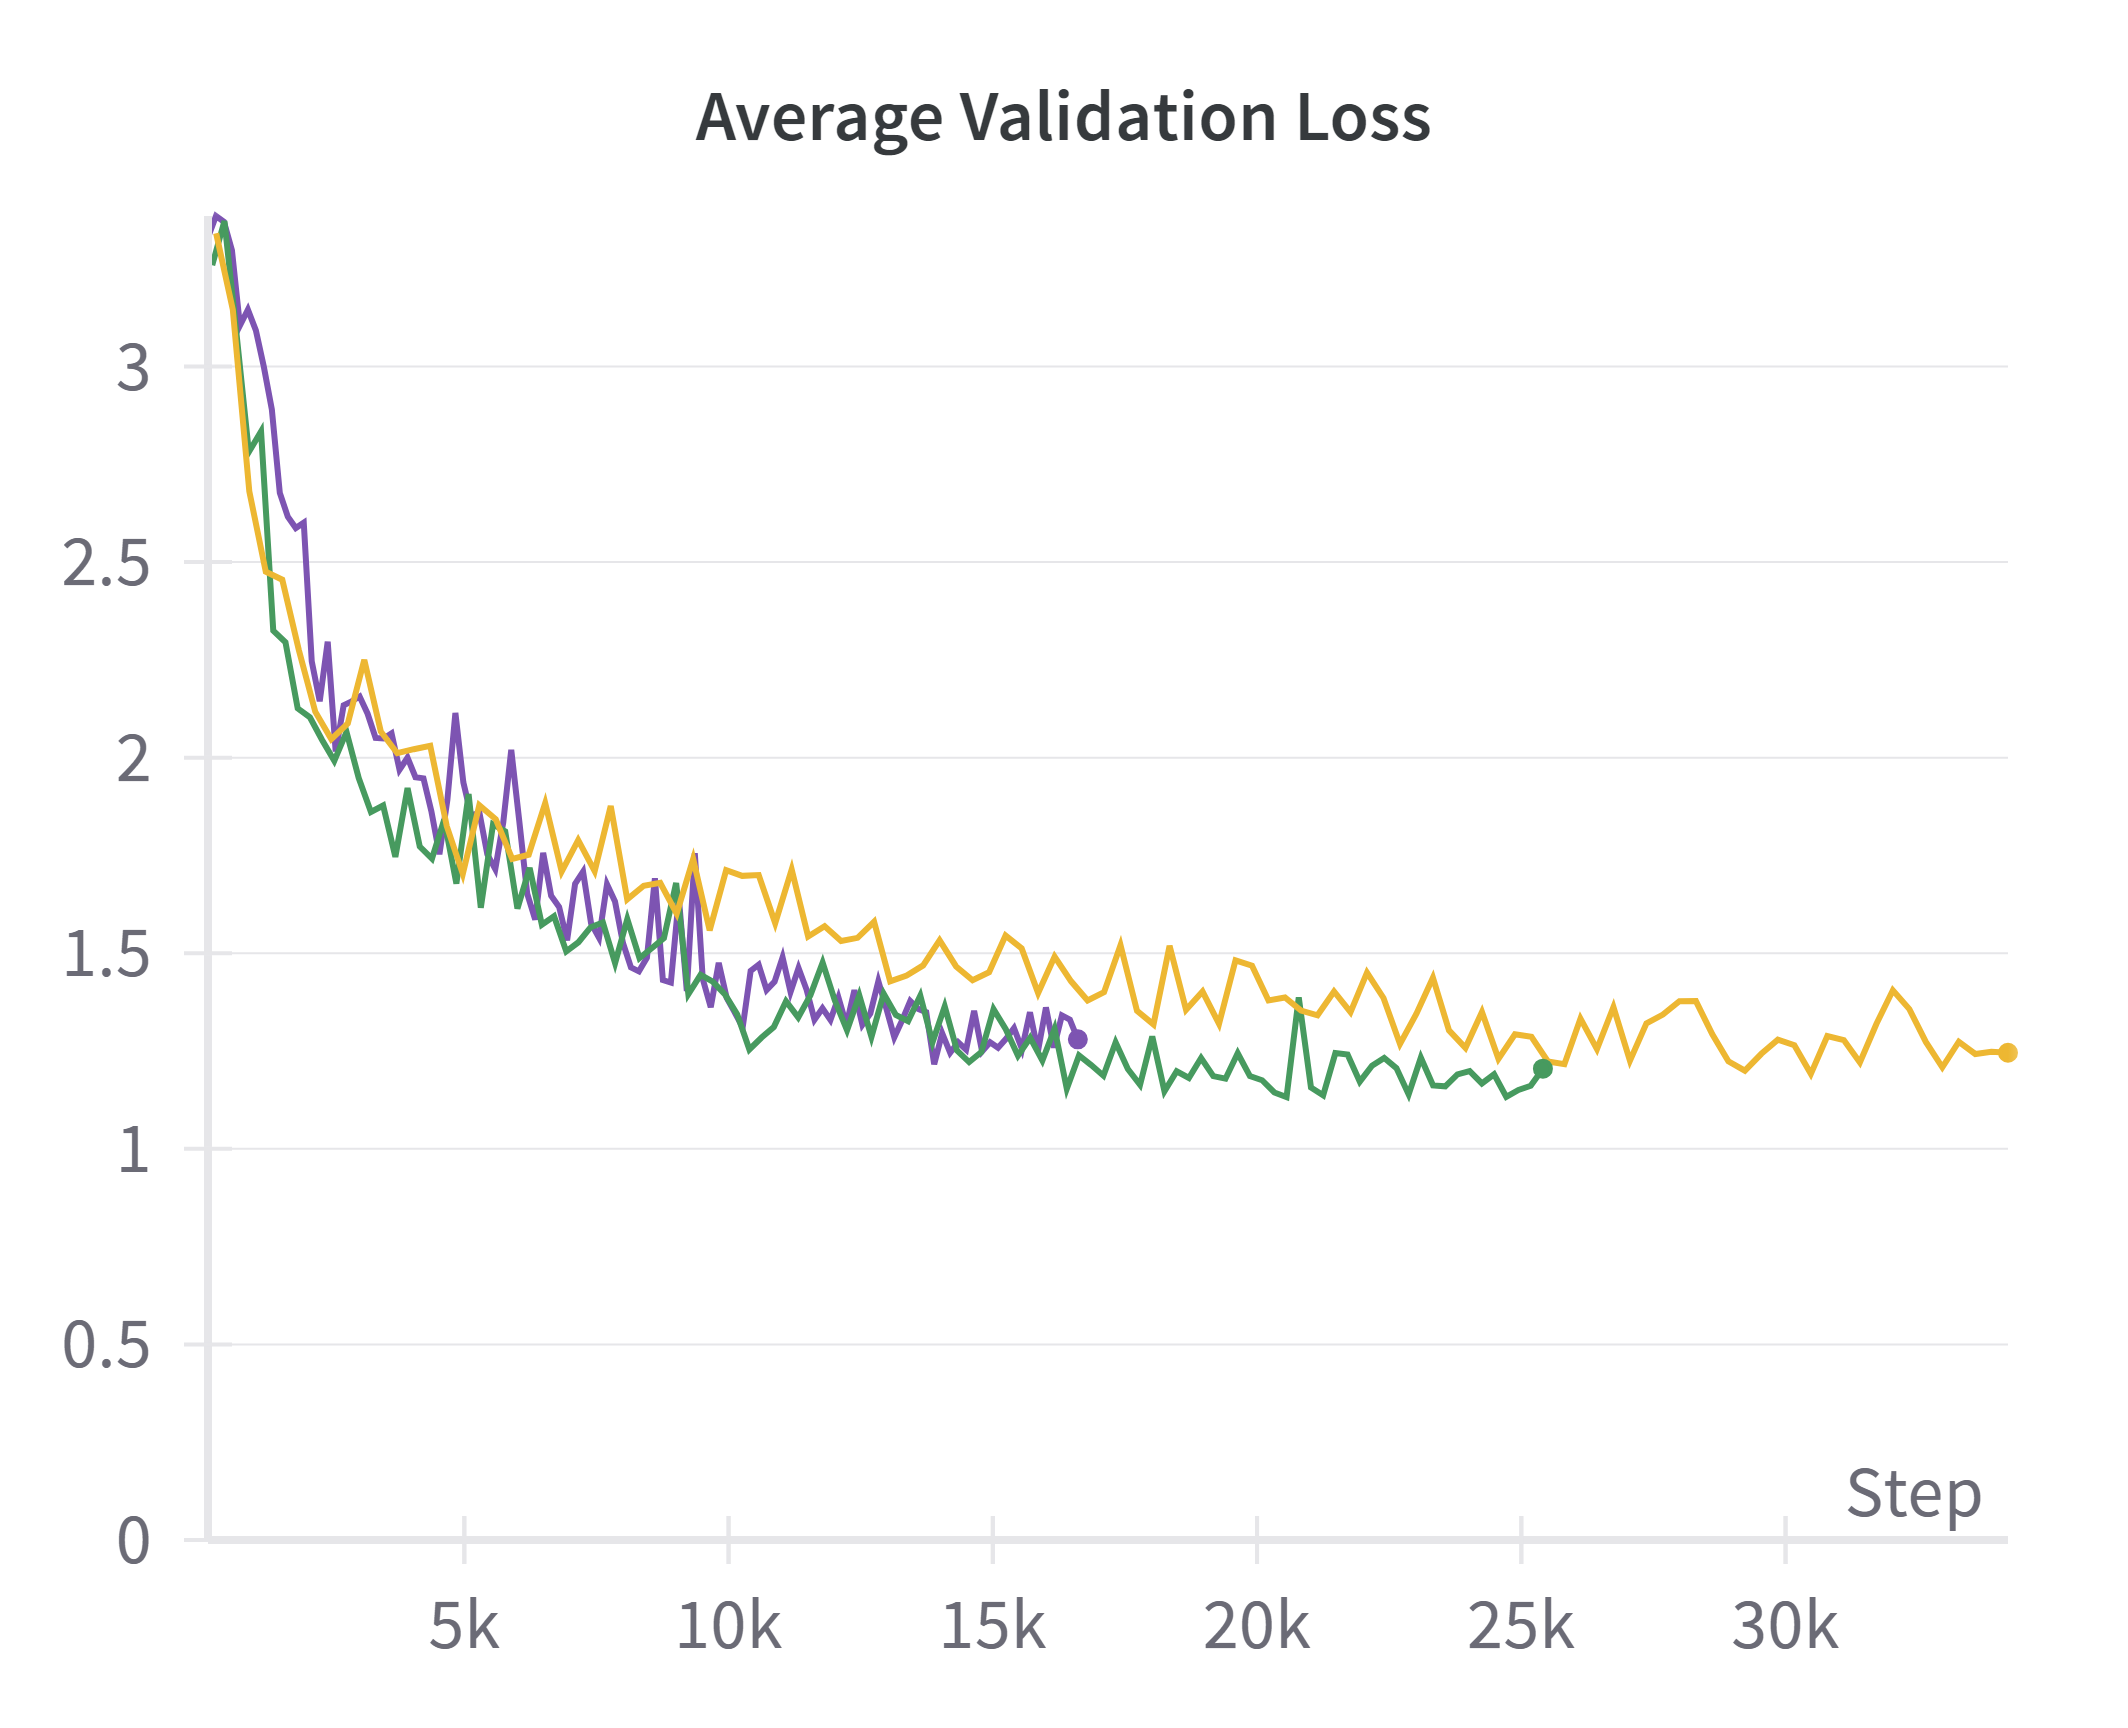
\includegraphics[width=0.5\textwidth]{figure_results_supcon-pre_avg-val-loss.png}
	\caption{Trainings- (links) und Validierungsfehler (rechts) während des Contrastive Pre-Trainings. Lila: Versuch 1, Grün: Versuch 2, Gelb: Versuch 3.}
	\label{fig:supcon-pre-loss}
\end{figure}

% Nur reale Daten
% Mit ID-Augmentationen
% Mit ID-Augmentationen und OOD-Augmentationen für hard-negative mining

\subsection{Lineare Klassifikation} \label{sec:supcon-lin-results}

Die Trainingskurven der linearen Klassifikation teilen sich auf in Trainings- und Validierungsfehler (siehe Abbildung \ref{fig:supcon-lin-loss}), Trainings- und Validierungsgenauigkeit (siehe Abbildung \ref{fig:supcon-lin-acc}) und die ID- und OOD-Confidence (siehe Abbildung \ref{fig:supcon-lin-ood-detection}).

\begin{figure}[h]
	\centering
	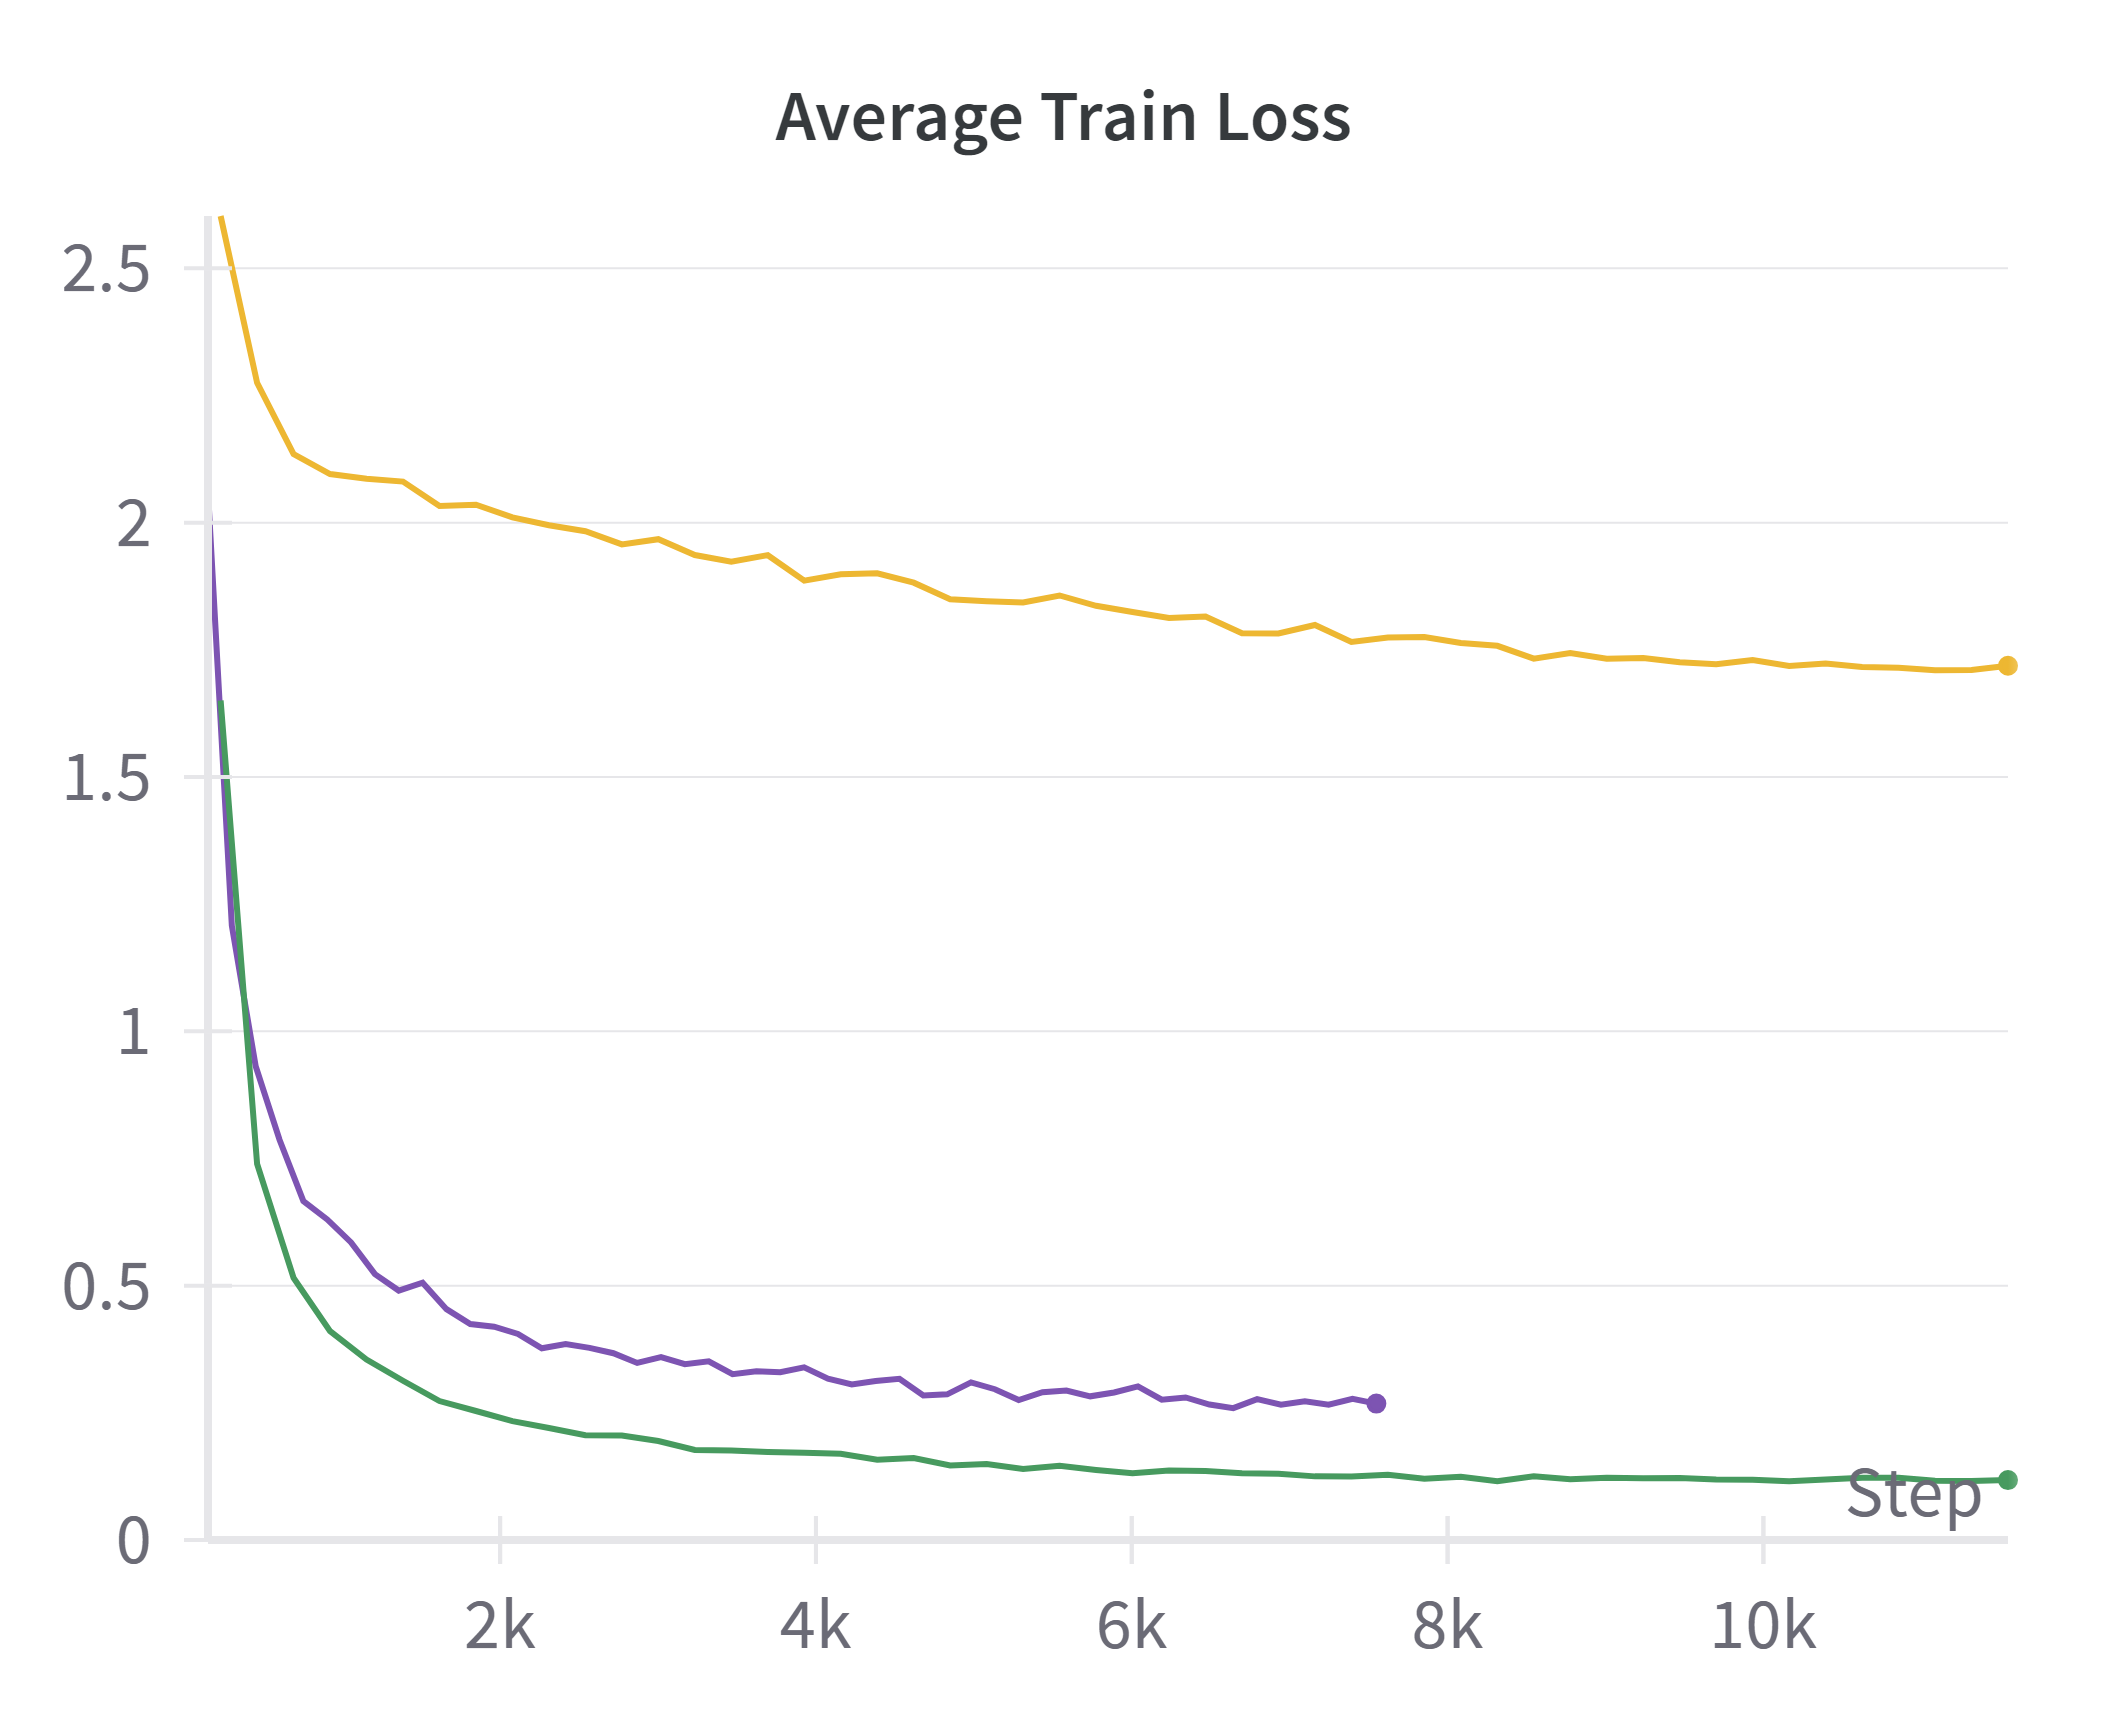
\includegraphics[width=0.5\textwidth]{figure_results_supcon-lin_avg-train-loss.png}%
	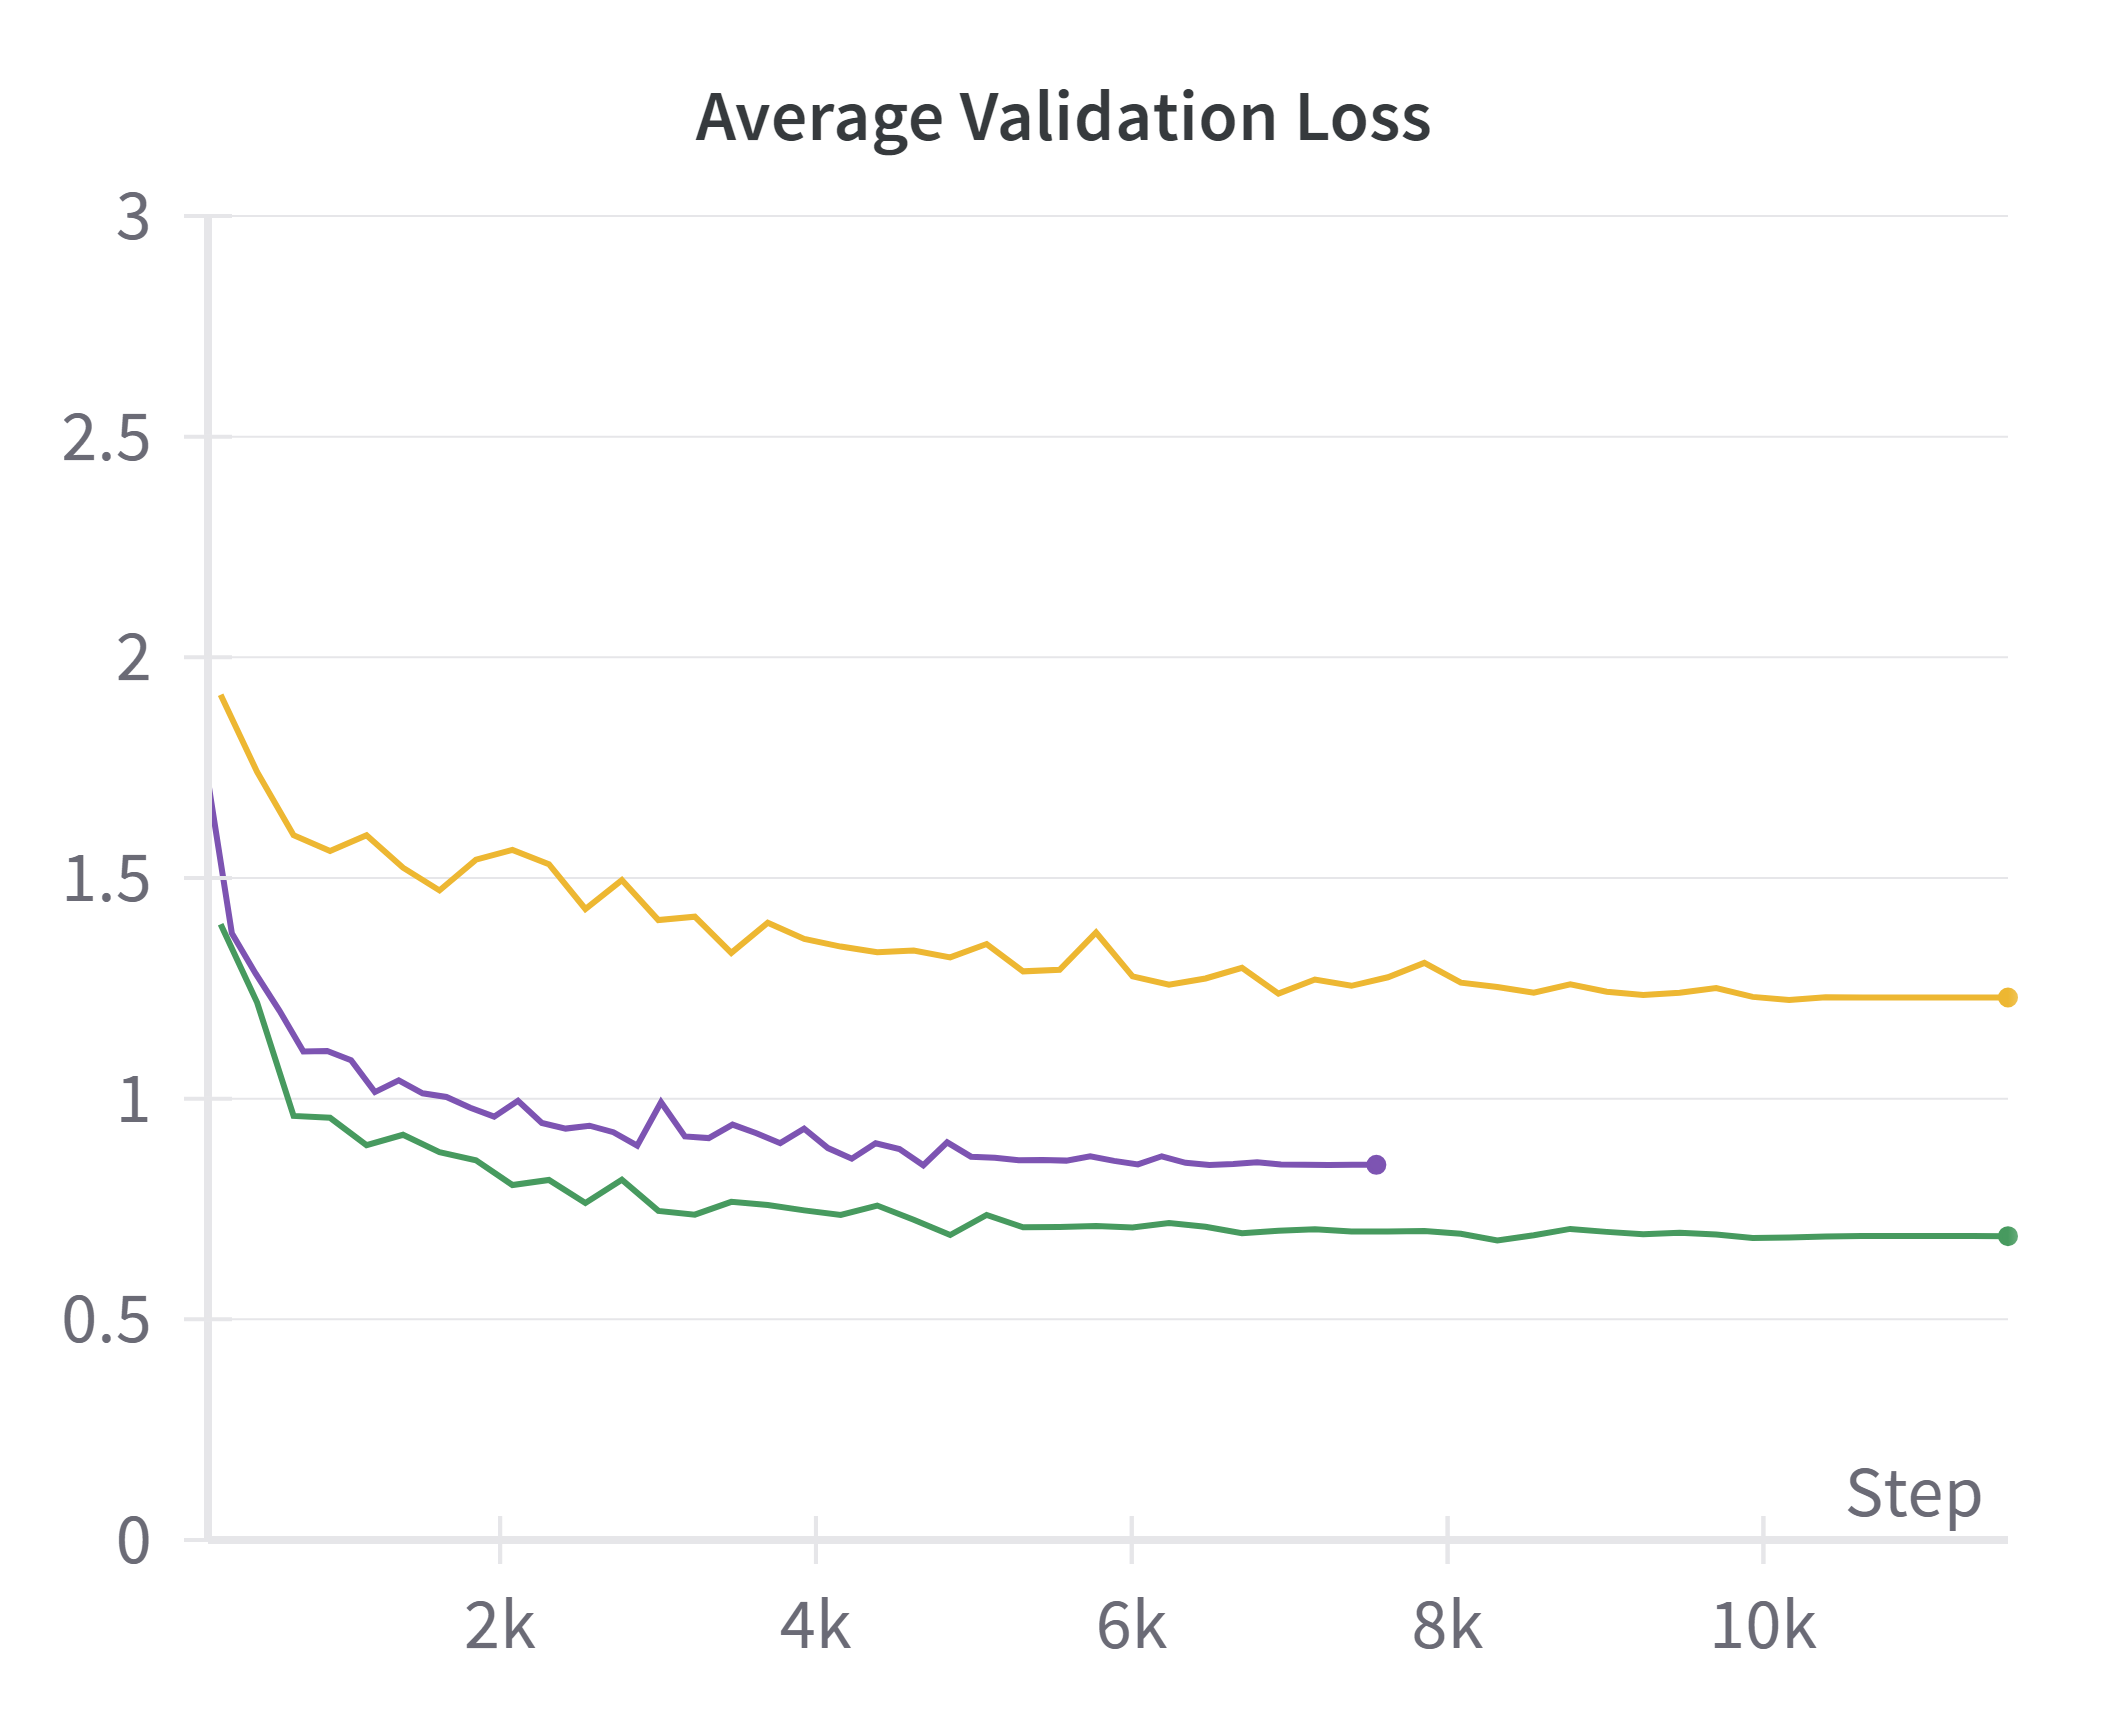
\includegraphics[width=0.5\textwidth]{figure_results_supcon-lin_avg-val-loss.png}
	\caption{Beispieltext 1}
	\label{fig:supcon-lin-loss}
\end{figure}
\begin{figure}[h]
	\centering
	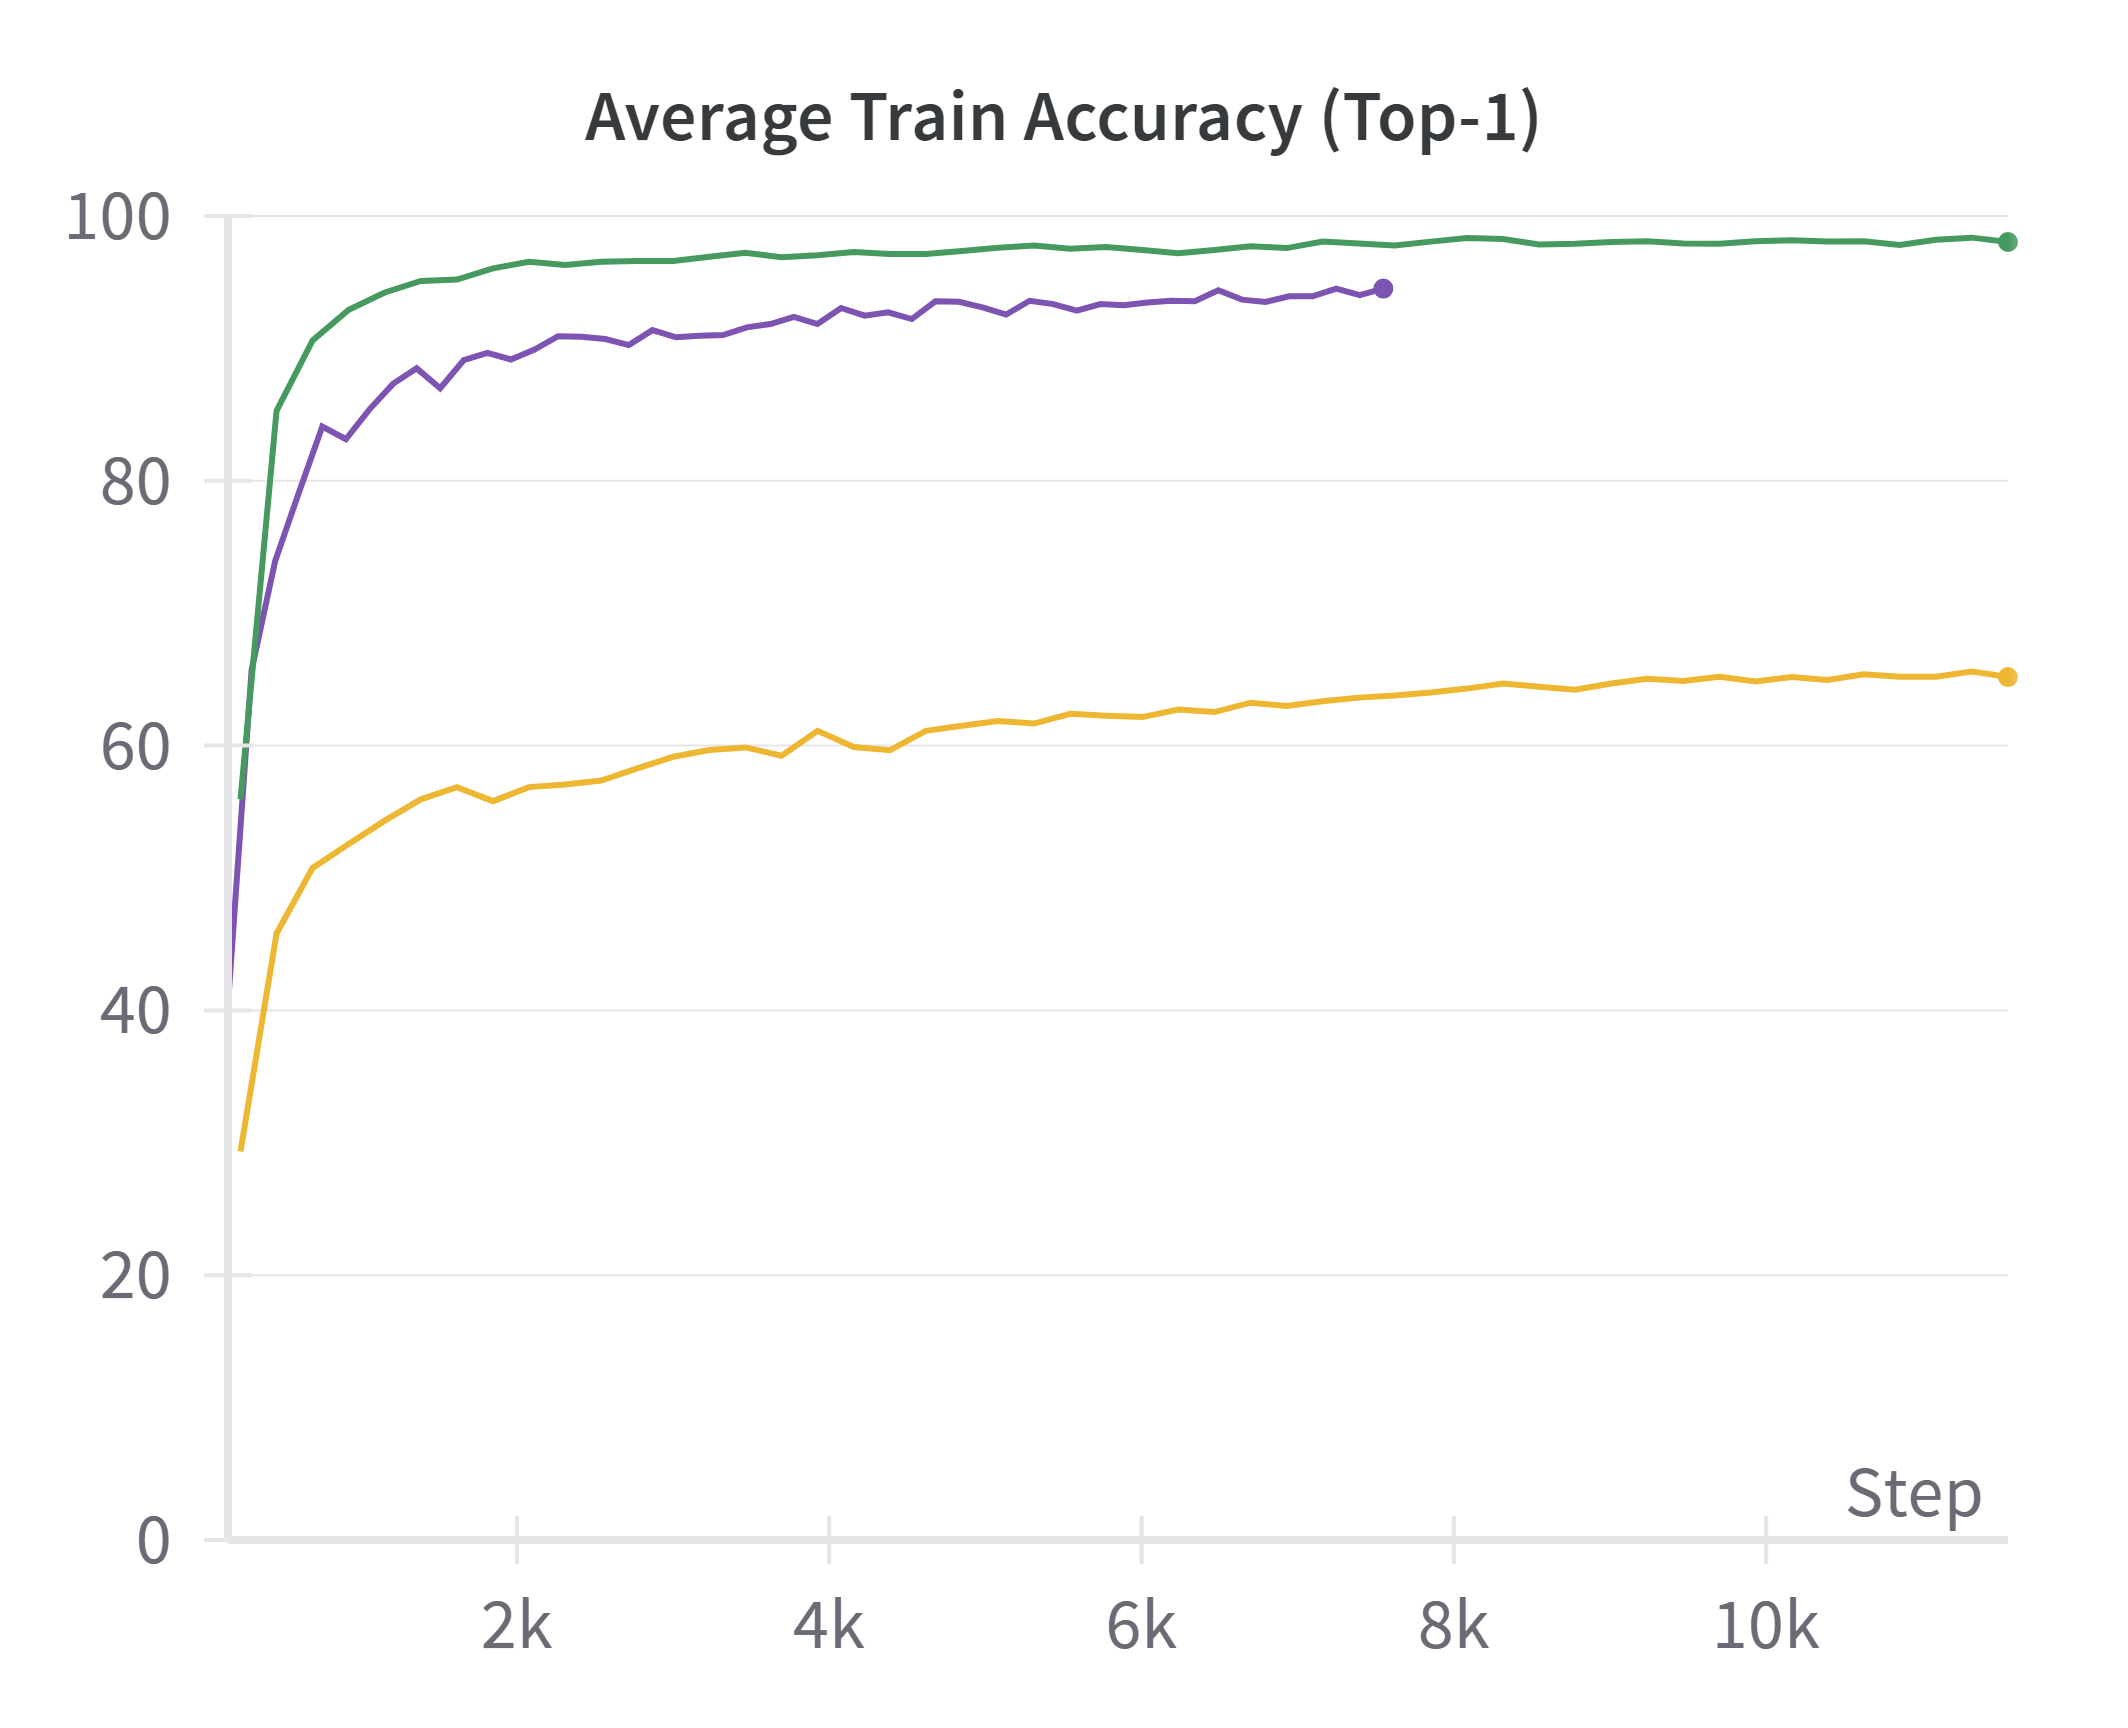
\includegraphics[width=0.5\textwidth]{figure_results_supcon-lin_avg-train-acc.png}%
	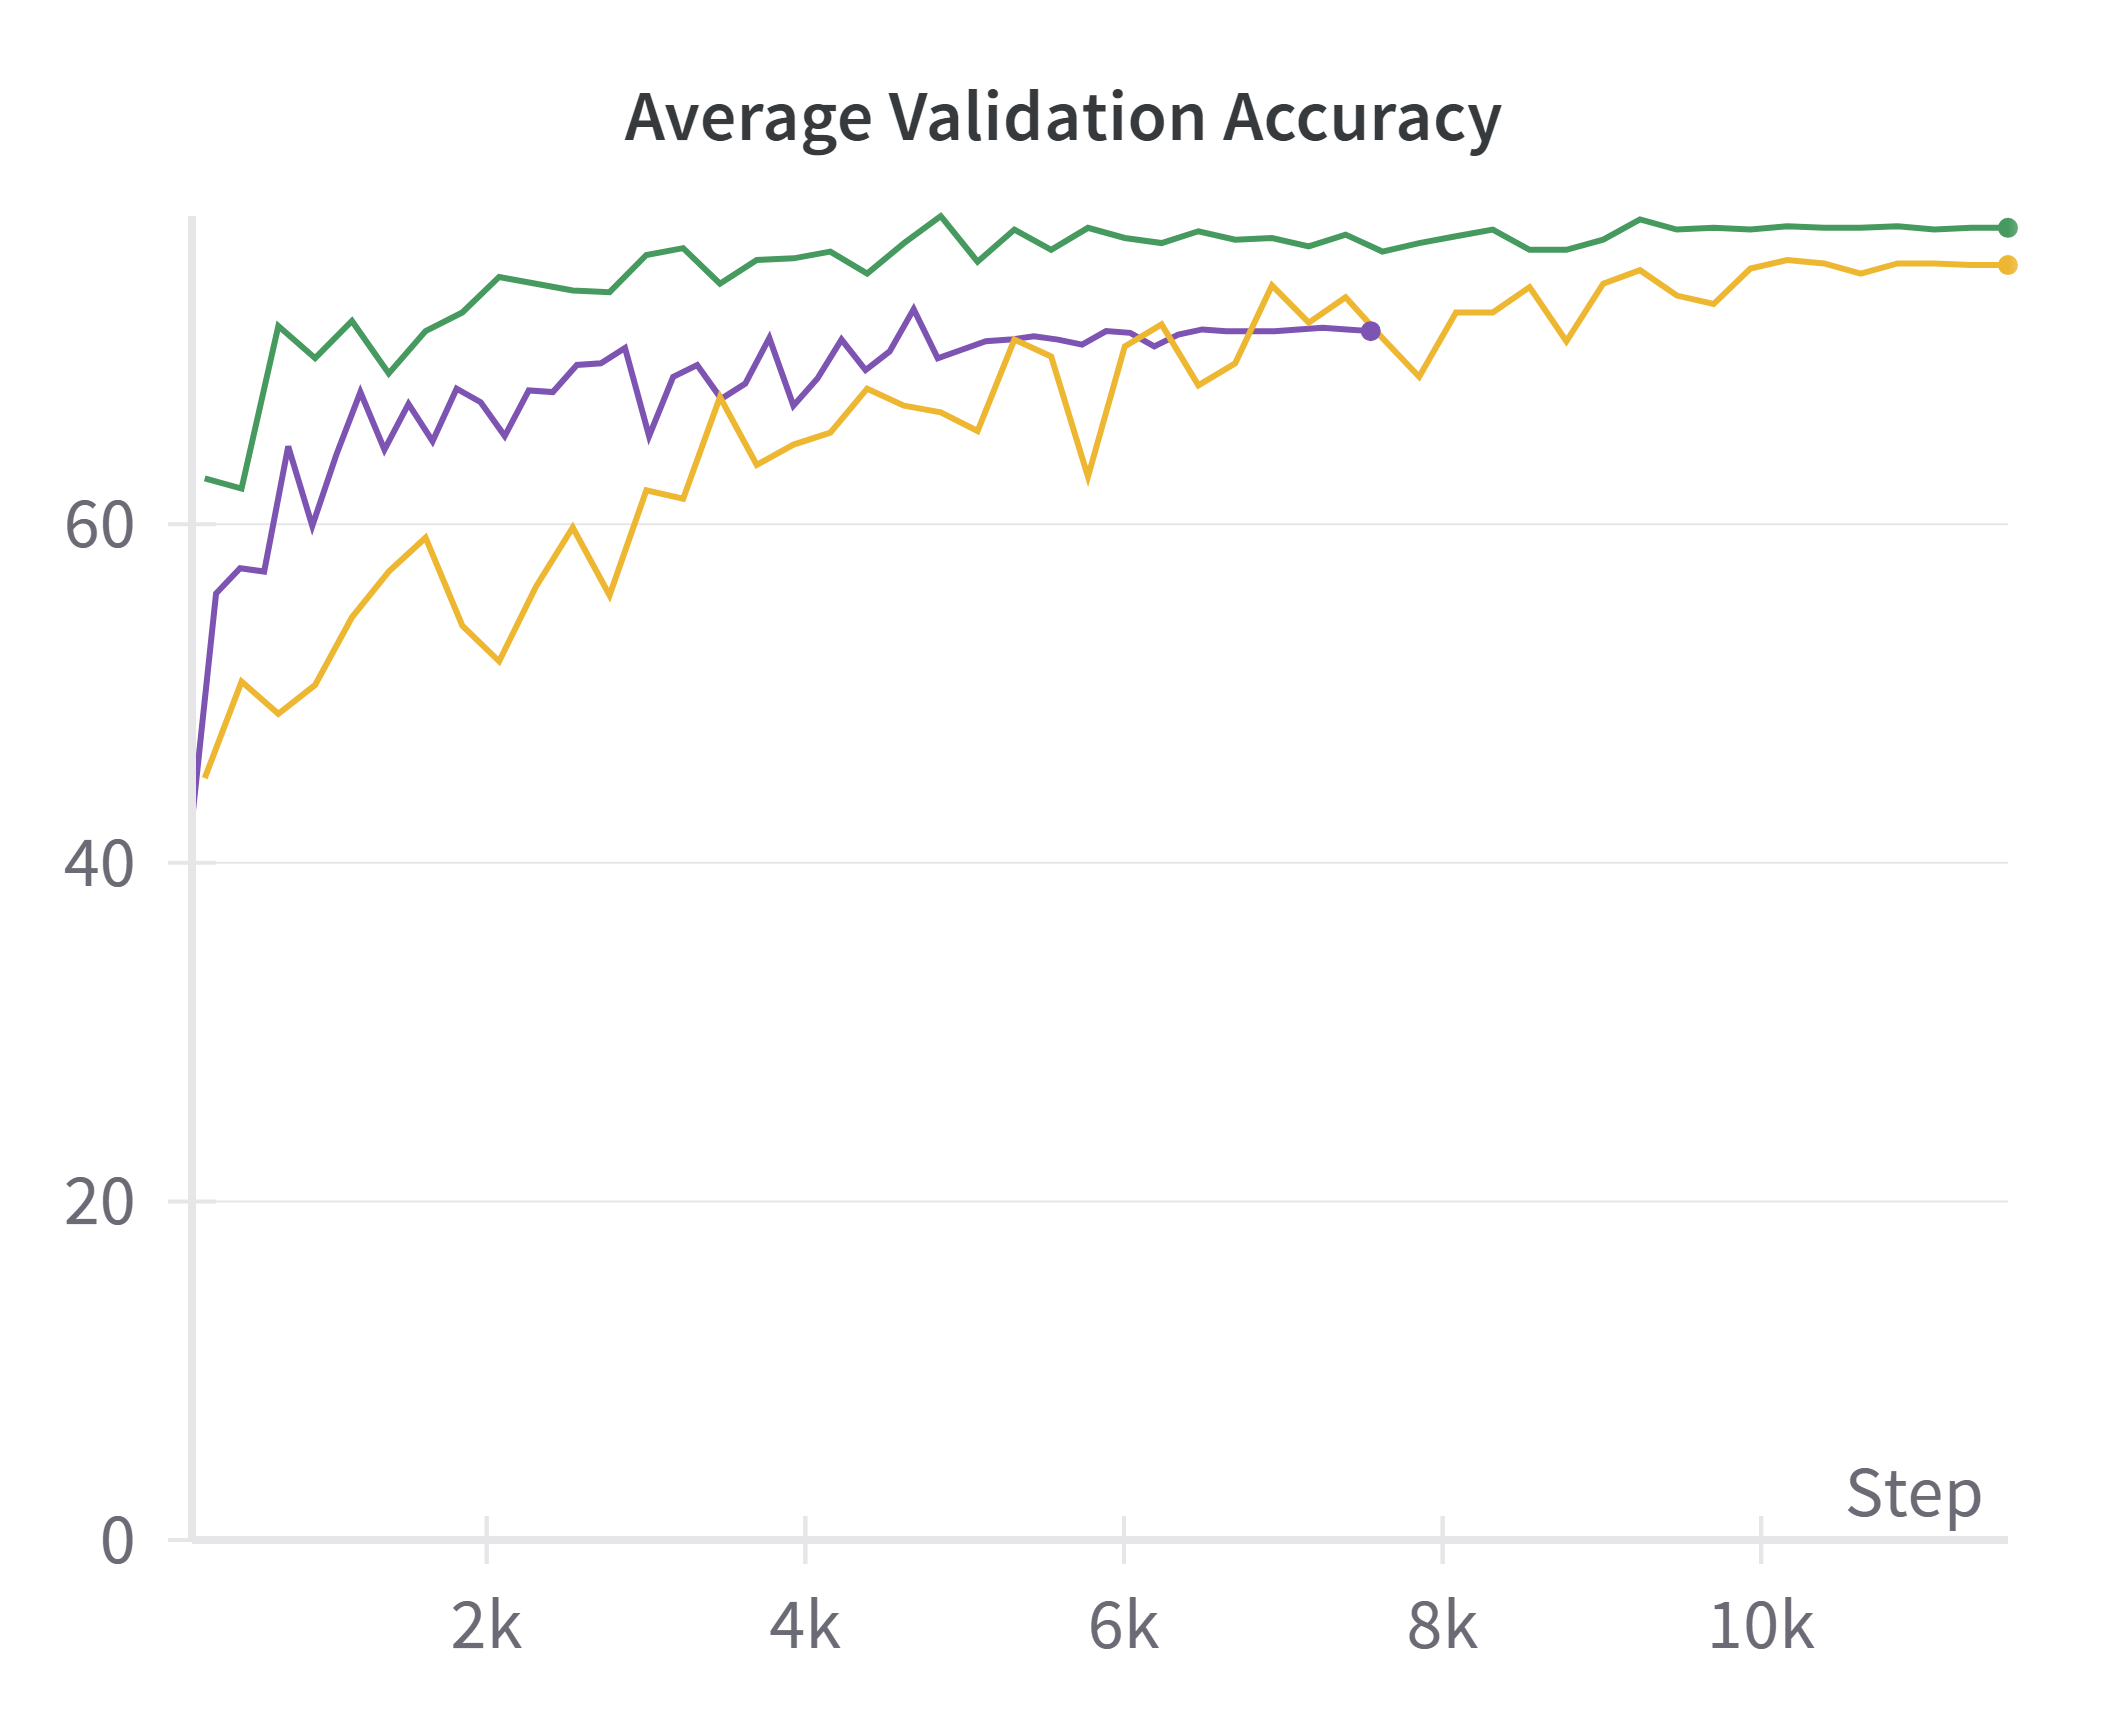
\includegraphics[width=0.5\textwidth]{figure_results_supcon-lin_avg-val-acc.png}
	\caption{Beispieltext 2}
	\label{fig:supcon-lin-acc}
\end{figure}
\begin{figure}[h]
	\centering
	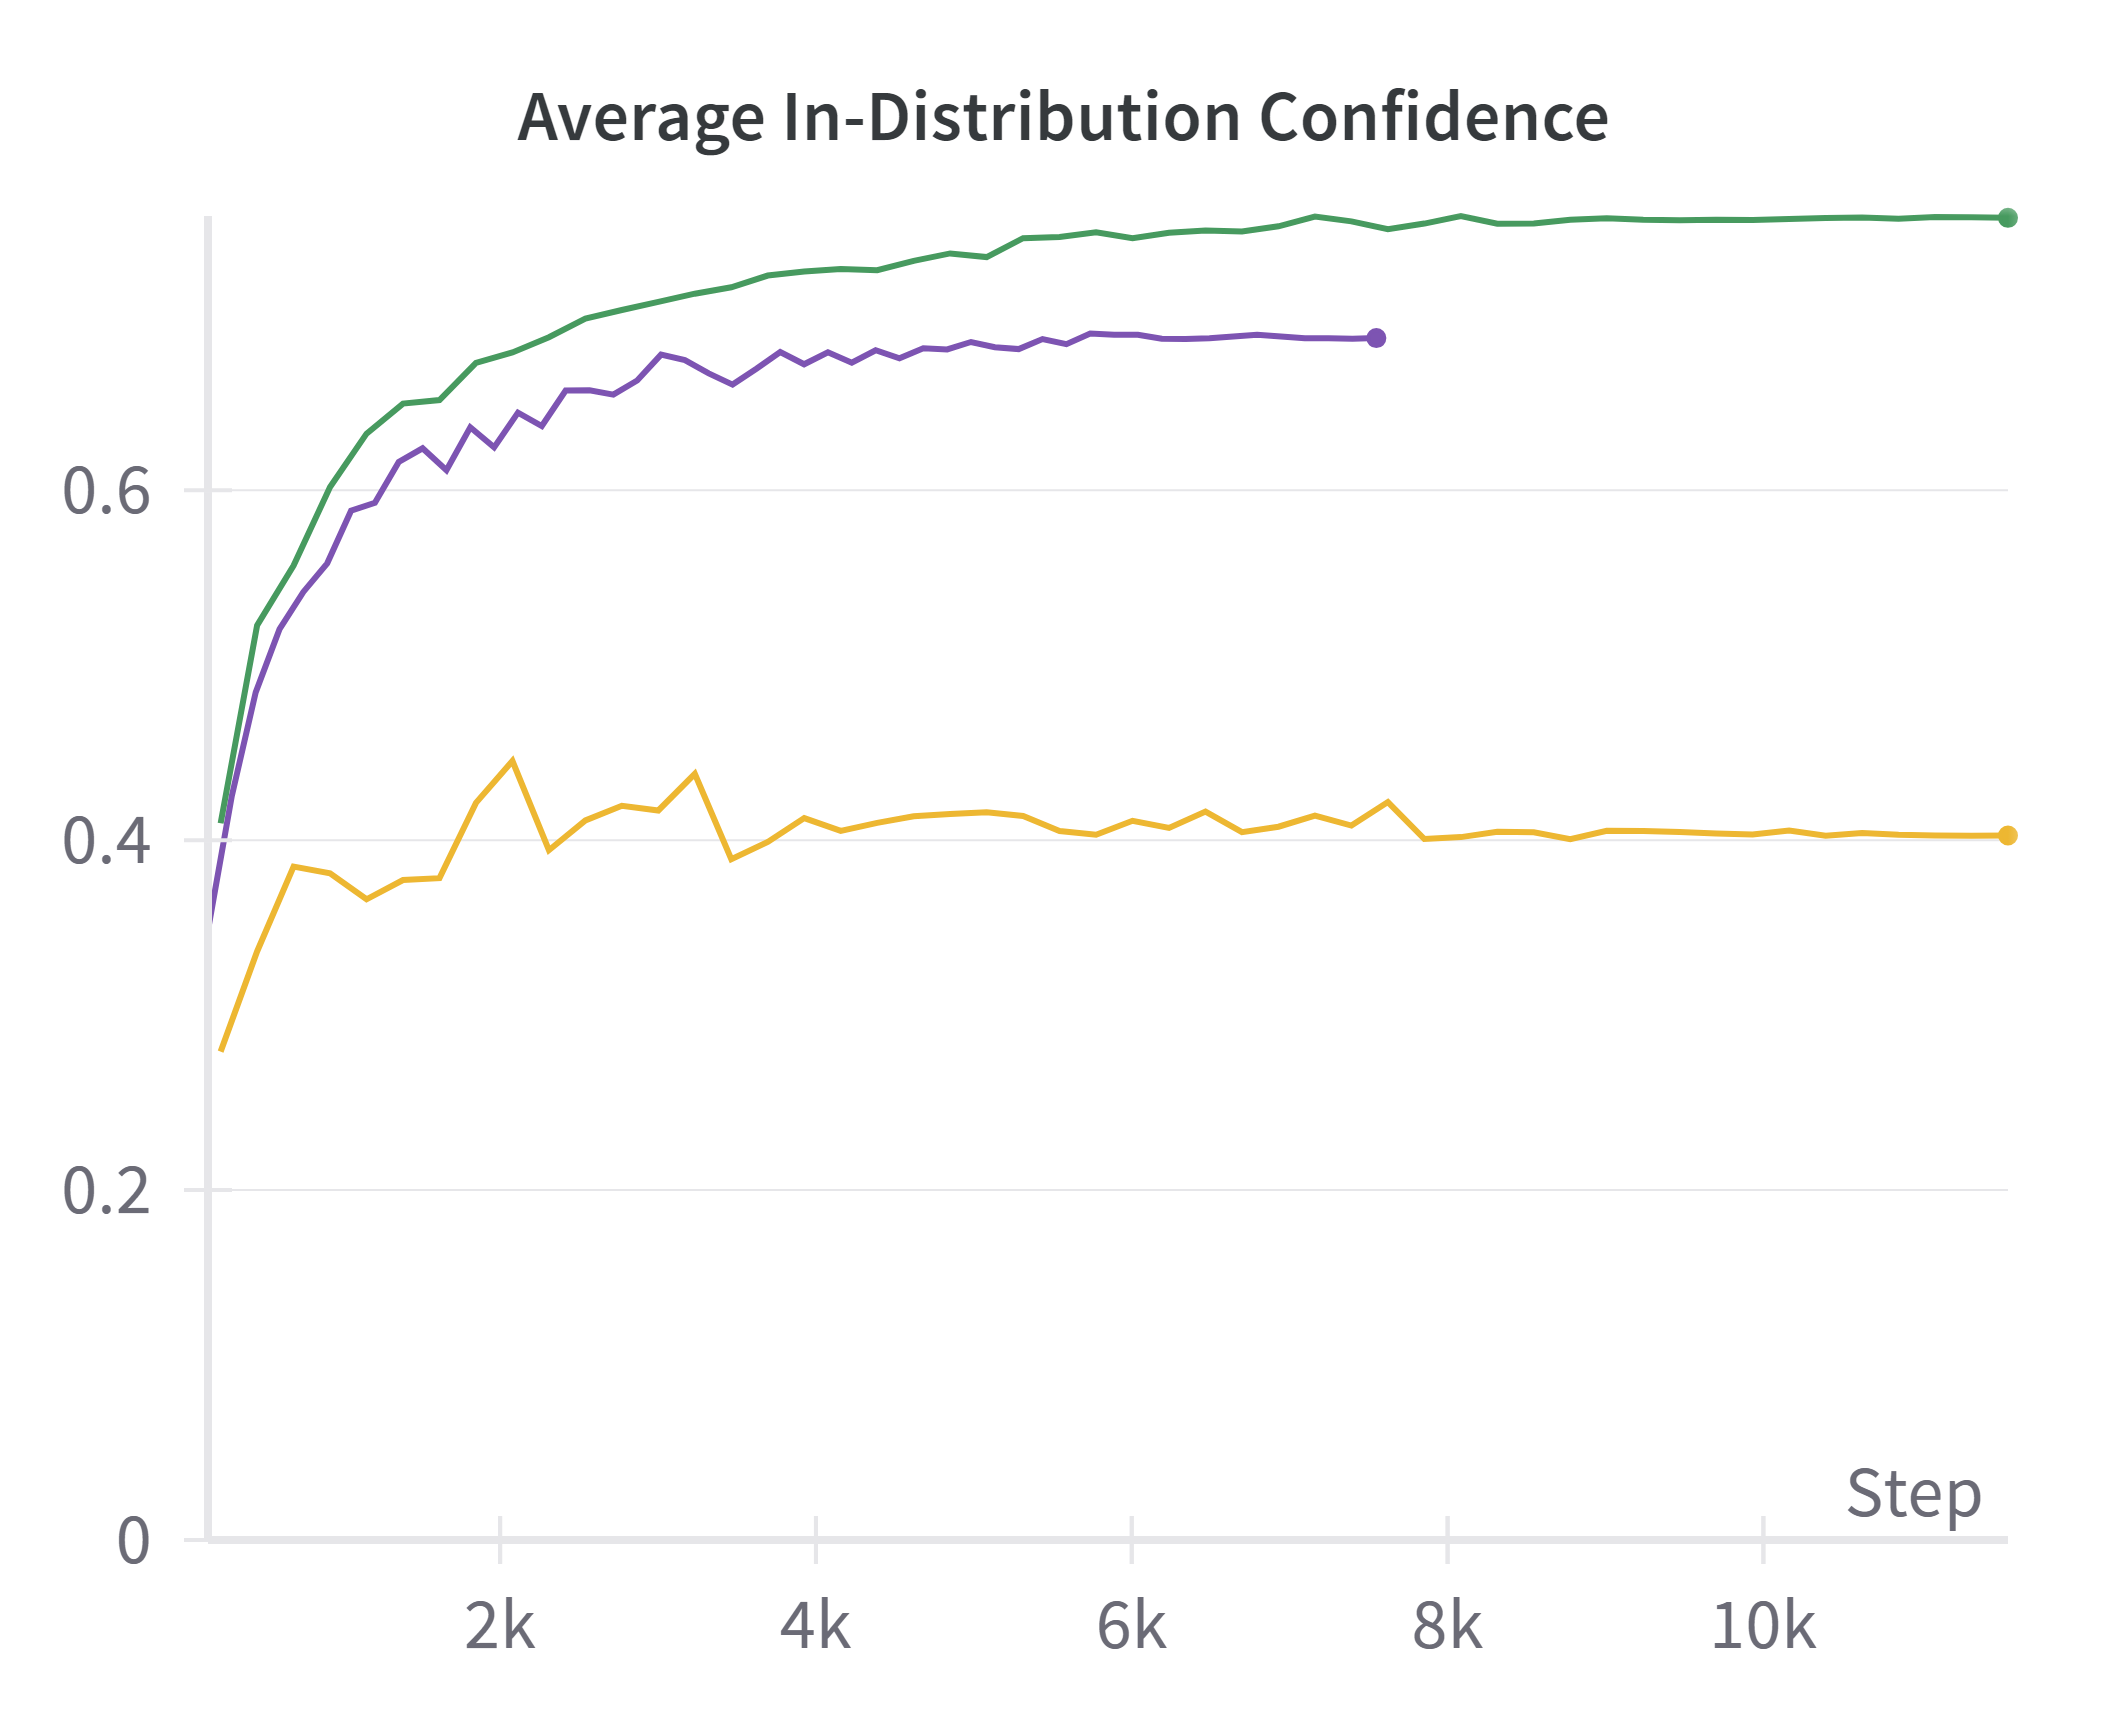
\includegraphics[width=0.5\textwidth]{figure_results_supcon-lin_avg-id-conf.png}%
	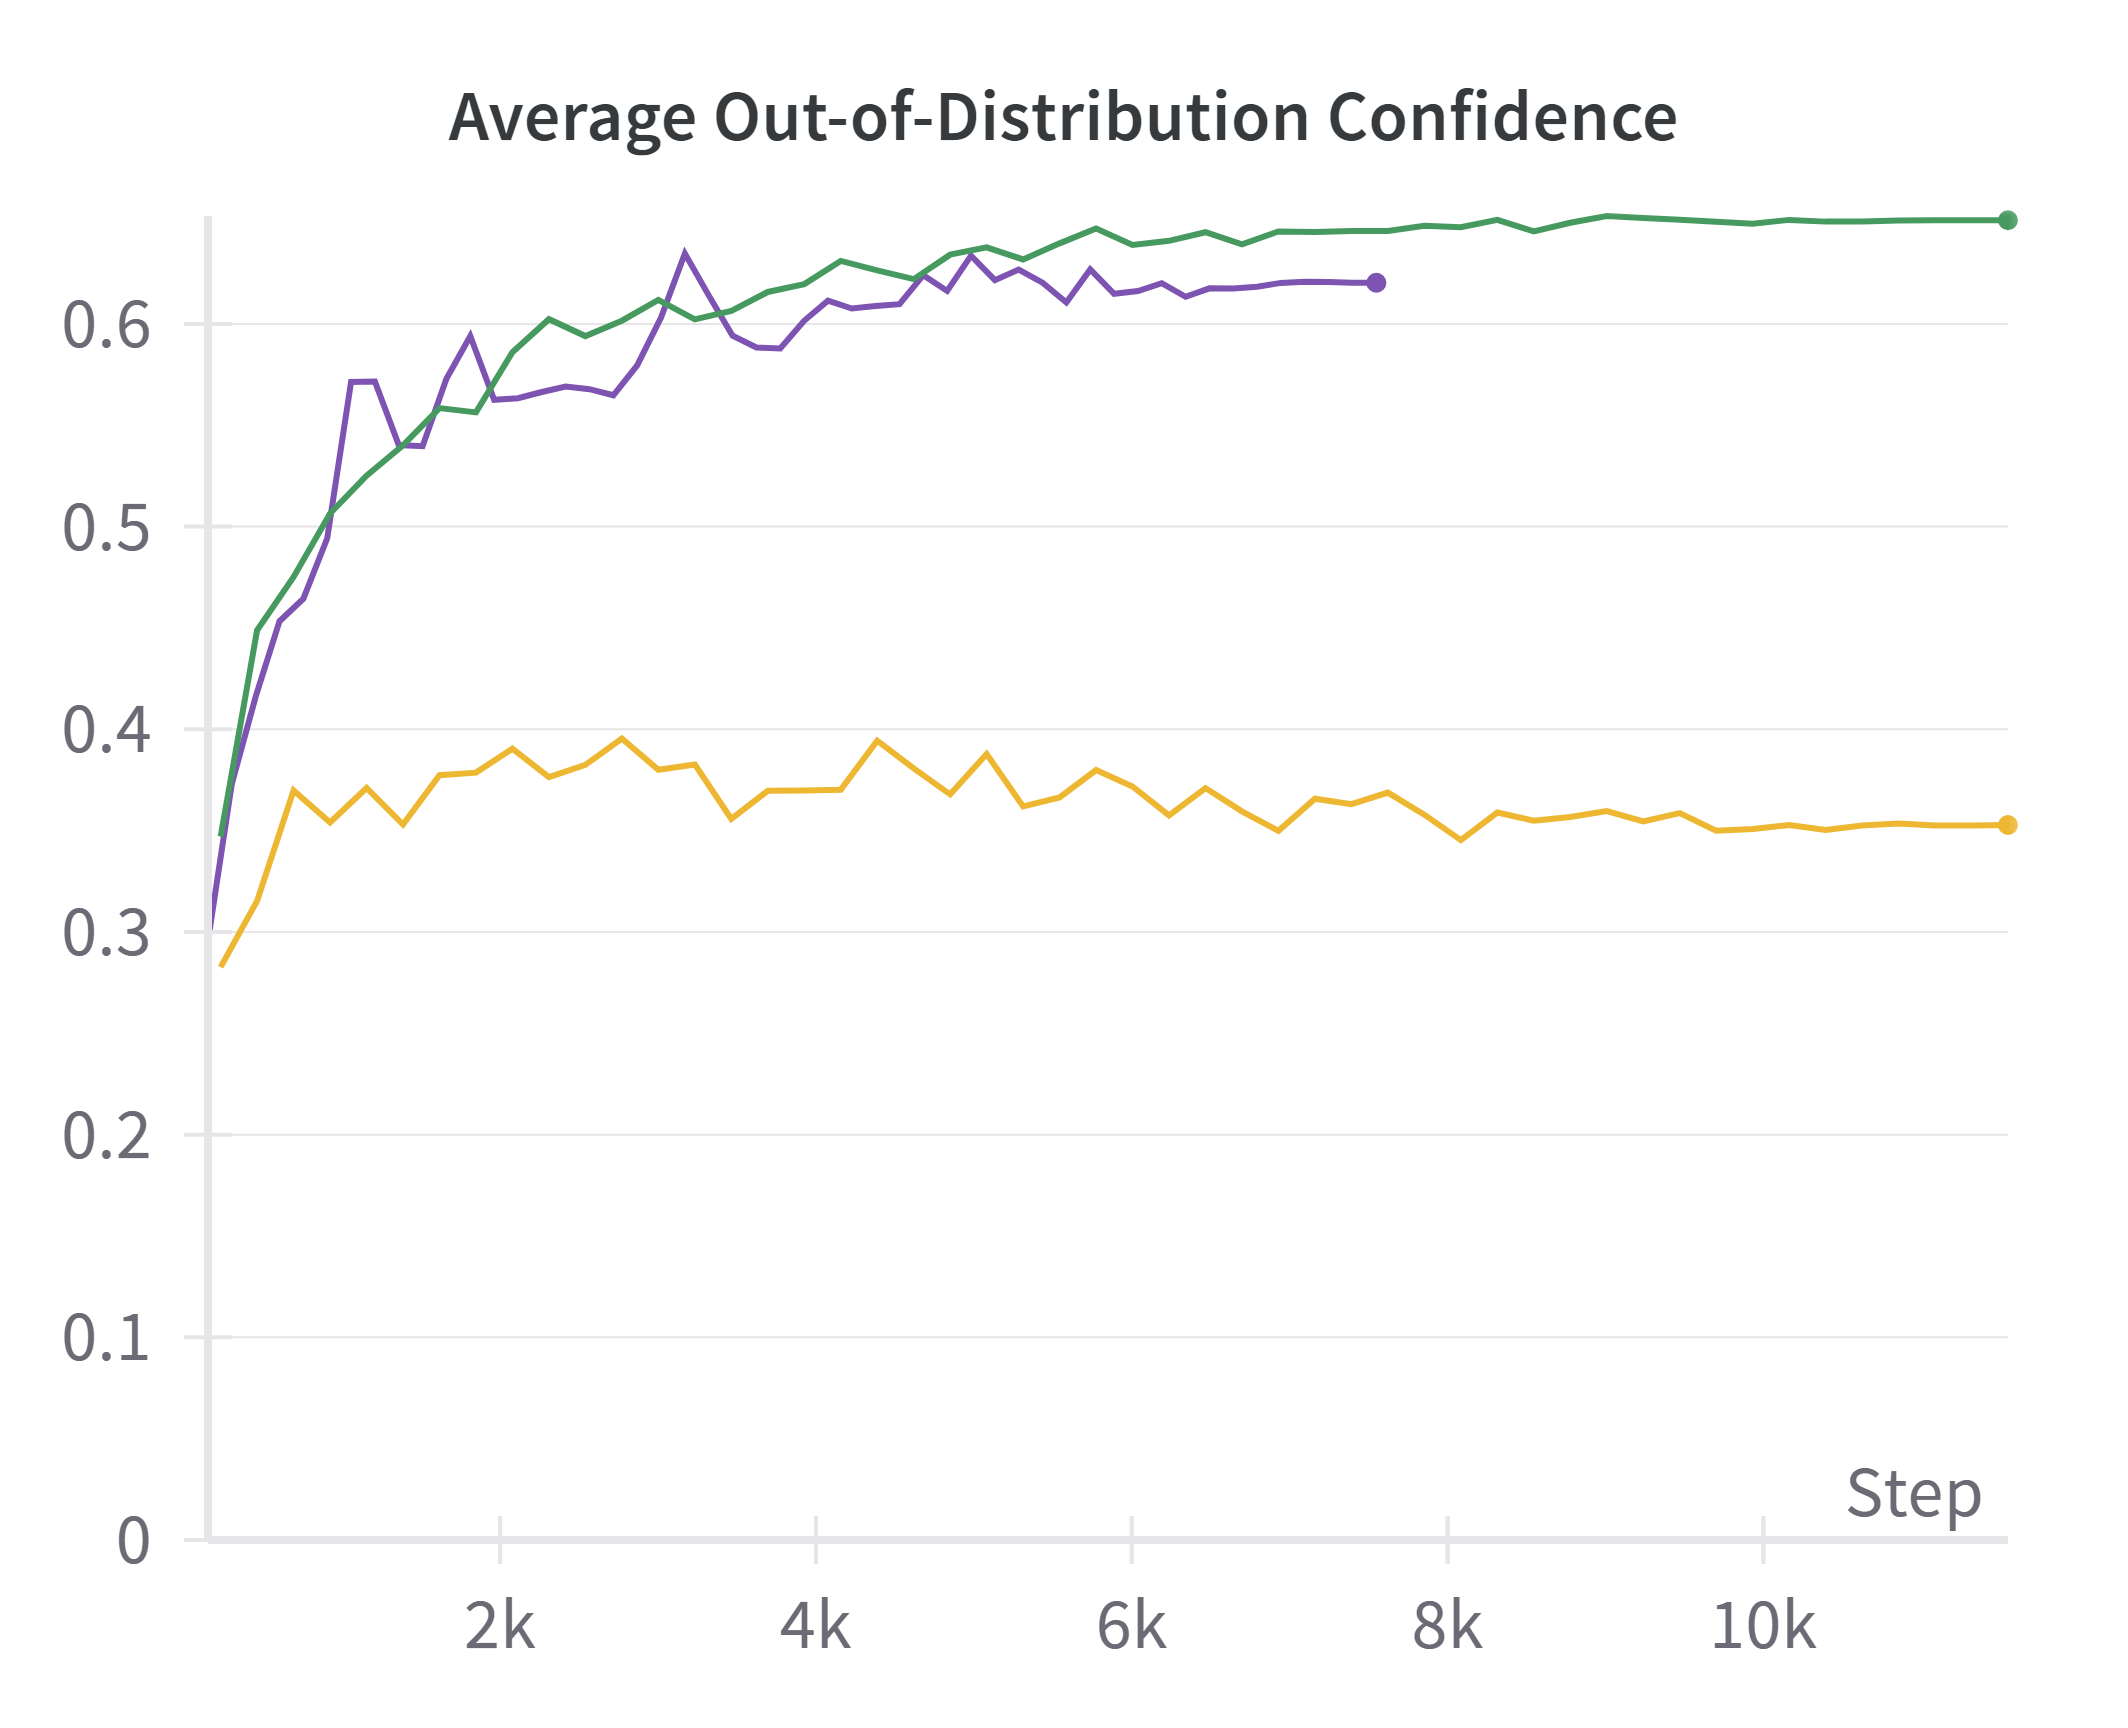
\includegraphics[width=0.5\textwidth]{figure_results_supcon-lin_avg-ood-conf.png}
	\caption{Beispieltext 3}
	\label{fig:supcon-lin-ood-detection}
\end{figure}

Die in Abschnitt \ref{sec:evaluation} definierten Metriken Accuracy, ID-Confidence und OOD-Confidence wurden für den letzten Validierungsschritt nach Ende des Trainings der linearen Klassifikation ausgelesen und sind in Tabelle \ref{tab:supcon-lin-results} aufgeführt.

\begin{table}[h]
	%\centering
	\caption{Testergebnisse der linearen Klassifikation.}
	\begin{tabular}{|c|c|c|}
		\hline
		\textbf{Versuch} & \textbf{Accuracy (\%)} & \textbf{ID-/OOD-Confidence (Differenz)} \\
		\hline
		1 & 71.4 & 0.69 / 0.62 (0.07) \\
		2 & 77.5 & 0.76 / 0.65 (0.11) \\
		3 & 75.3 & 0.40 / 0.35 (0.05) \\
		\hline
	\end{tabular}
	\label{tab:supcon-lin-results}
\end{table}

\section{Vergleich der Ergebnisse} \label{sec:results-comparison}

% Einleitung
Als Grundlage für die Diskussion und Beantwortung der Forschungsfragen werden die Ergebnisse mit und ohne In-Distribution- und Near Out-of-Distribution-Augmentationen verglichen. Es wird auf die Klassifikations-Performance (Accuracy) und die Out-of-Distribution-Detektion (ID-/OOD-Confidence) eingegangen.

\subsection{Mit und ohne In-Distribution-Augmentationen} \label{sec:results-comparison-id}

...

\subsection{Mit und ohne Near Out-of-Distribution-Augmentationen} \label{sec:results-comparison-ood}

...
